\chapter{Experiential Learning of Networking Technologies}

\vskip -15pt

\centerline{{\LARGE\sl Understanding IP Routing}}


\vskip 0.8cm

\begin{center}
{\large\uppercase{$\text{Ram P. Rustagi}$}} 


\vskip -6pt

\end{center}

\vskip 2cm




\vfill




\newpage

\begin{multicols}{2}

In the previous article \cite{art2-key01}, we have studied assignment of IP address \cite{art2-key02} to a host, and its role in connecting to internet and communicating with other devices. We explored concept of a network number which is determined using IP address and subnet mask. When network number of two hosts is same, then these two hosts belongs to same network else these hosts belong to different networks. Hosts within the same network communicate directly with each other whereas hosts belonging to different network communicate using one or more intermediate routers. A router connects two networks, and its main job is to receive packets from one network and forward it to another network so as to enable the packet delivery towards its final destination. When two hosts are connected by many intermediate networks, communication between these two hosts require that each of the intermediate router in the path forward the packet on to the network which is closer to the destination and router in the last leg of this path will deliver the packet to destination host. In this article, we will explore this concept of packet forwarding and the mechanisms used to achieve this packet forwarding.

Consider the connectivity of two networks, say Network-1 and Network-2, as shown in Figure~\ref{chap2-fig01}. Each of these two networks consists of many connected systems (though as a representation only 2 are shown). Host ${\rm H}_1$ and ${\rm H}_2$ are part of Network-1, and Host ${\rm H}_3$ and ${\rm H}_4$ are part of Network-2. These two networks are connected via many intermediate routers, which we can consider as representing the internet. Host H1 and ${\rm H}_2$ belongs to same network 10.x.x.0/24, and hence can communicate directly without requiring any intermediate router. Similarly, host ${\rm H}_3$ communicates directly with ${\rm H}_4$ as both belong to same network 10.y.y.0/24. However, when ${\rm H}_1$ needs to communicate with ${\rm H}_3$, the packets have to go through all the intermediate routers. When ${\rm H}_1$ wants to send a packet to ${\rm H}_3$, it will forward the packet to router ${\rm R}_1$, which in turn will forward the packet to next router ${\rm R}_2$, and so on, and finally Router ${\rm R}_{\rm n}$ will deliver the packet to host ${\rm H}_3$. Thus, communication between two hosts involves routing of packets and primary focus of this article is to explore the mechanism used in forwarding these packets.
\end{multicols}

\begin{figure}[H]
\centering
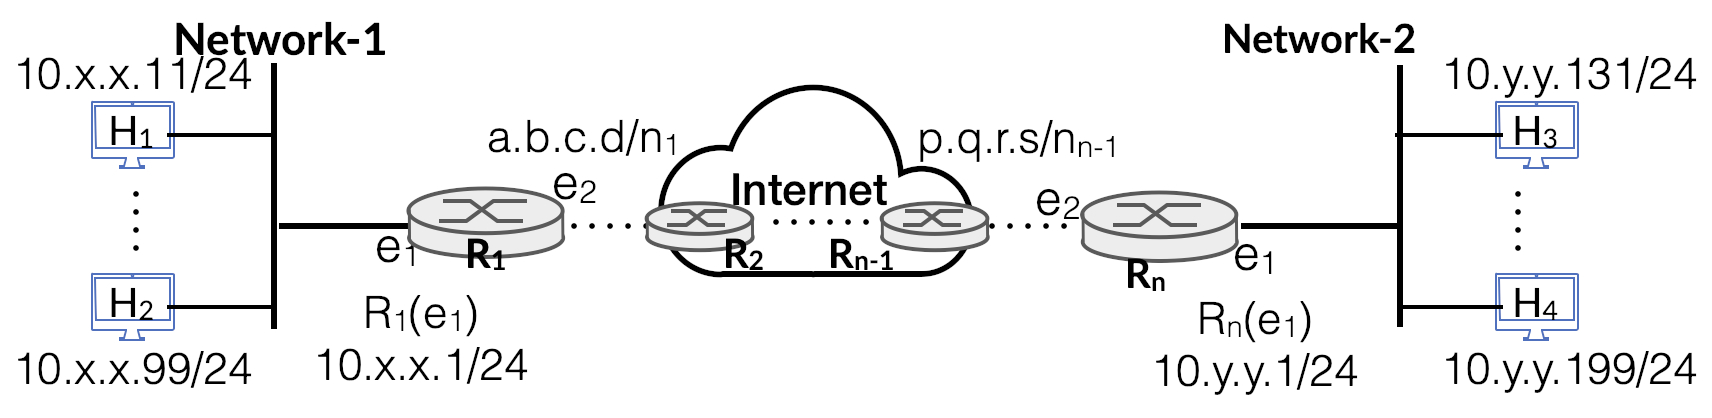
\includegraphics[scale=1.25]{src/Figures/chap2/chap2-fig01.jpg}
\caption{Connectivity of two Networks, each network having many systems in it}\label{chap2-fig01}
\end{figure}

\begin{multicols}{2}
Whenever, a host needs to send a packet to another hosts, it must know the IP address of destination host. For example, when we use browser to search at google.com, the machine where browser is running, finds the IP Address of gogole.com and then sets up TCP connection using IP address of google.com. When sending a packet, a host consults its routing table (also called as forwarding table) and determine the next hop in the path to destination host. Entries in the routing table plays a crucial role in how a host makes a packet forwarding decision. The routing decision using the routing table is always required irrespective of whether the destination host is in the same network or a different network.

\section{Routing Table Structure}\label{chap2-sec-1}

\vskip -.2cm

The main purpose of routing table is to help a host in determining the next hop where packet should be forwarded. The next hop could even be the next intermediate router or the final destination host itself. At its core, routing table has following four column fields, though in many implementations it may have some more information fields, such as cost metric etc., which we will not consider for our discussion.
\begin{itemize}
\item[i.] Destination Network.
\item[ii.] Subnet mask (for destination network).
\item[iii.] Network interface.
\item[iv.] Next hop or gateway router’s IP address.
\end{itemize}

A routing table would have number of row entries, with each row corresponding to a destination network. First two fields together identify a network, and are used to check if destination IP address of packet belongs to this network. If this entry matches, then packet is forwarded on the associated interface ($3^{\rm rd}$ field) to the next hop ($4^{\rm th}$ field). Next hop entry field is applicable when destination host is not connected to local network and identifies the IP address of next router in the forward path.  A typical set of entries for router $\rm{R}_1$ in Figure.~\ref{chap2-fig01} is given below in Table~\ref{chap2-table-1}, and routing entries for Host $\rm{H}_1$ is given in Table~\ref{chap2-table-2}.
\end{multicols}

\vskip -.8cm

\begin{table}[H]
\caption{Routing entries for ${\rm R}_{1}$}\label{chap2-table-1}
\begin{center}
\begin{tabular}{|c|m{3.7cm}|m{1.5cm}|m{1.5cm}|m{2.5cm}|}
\hline
\textbf{S.N} & \textbf{Destination Network} & \textbf{Netmask} & \textbf{Interface} & \textbf{Next Hop}\\
\hline
1 & 10.x.x.0 &/24 & $\rm{e}_{1}$ & -\\
\hline
2 & a.b.c.d &/$\rm{n}_{1}$ & $\rm{e}_{2}$ & -\\
\hline
3 & \dots & \dots & \dots & \dots\\
\hline
4 & p.q.r.s & /$\rm{n}_{\rm{n}-1}$ & $\rm{e}_{2}$ & IP address of $\rm{R}_{2}$\\
\hline
5 & 10.y.y.0 & /24 & $\rm{e}_{2}$ & IP address of $\rm{R}_{2}$\\
\hline
6 & 0.0.0.0 & /0 & $\rm{e}_{2}$ & IP address of $\rm{R}_{2}$\\
\hline
\end{tabular}
\end{center}
\end{table}

\vskip -1cm

\begin{table}[H]
\caption{Routing entries for Host $\rm{H}_{1}$}\label{chap2-table-2}
\begin{center}
\begin{tabular}{|c|m{3.7cm}|m{1.7cm}|m{1.7cm}|m{2cm}|}
\hline
\textbf{S.N.} & \textbf{Destination Network} & \textbf{Netmask} & \textbf{Interface} & \textbf{Next Hop}\\
\hline
1 & 10.x.x.0 & /24 & Ethernet & -\\
\hline
2 & 0.0.0.0 & /0 & Ethernet & 10.x.x.1\\
\hline
\end{tabular}
\end{center}
\end{table}

\begin{multicols}{2}
First two entries in Table~\ref{chap2-table-1} corresponds to two networks to which router $\rm{R}_{1}$ is directly connected and hence there is no next hop address. These will be followed by number of entries corresponding to network numbers that exist in the network. The entries in $4^{\rm th}$ and $5^{\rm th}$ row correspond to two networks connected with the router $\rm{R}_{n}$. Lastly, there is an entry corresponding to 0.0.0.0/0 which is also referred to as default route entry. Use of this default entry is explained ahead. For any host which is typically connected to a single network, there are generally two entries, as shown in Table~\ref{chap2-table-2} for host $\rm {H}_{1}$. One entry corresponds to local network and other entry corresponds to default network i.e. 0.0.0.0/0. These entries are sorted in the decreasing order of number of bits in netmask. For example, entry for netmask /27 will come before entries of netmask /26 or /25 etc.

\section{Using Routing Table to Forward Packets}\label{chap2-sec2}

When a host needs to send a packet to destination host or an intermediate router need to forward a received packet, then both the host and the router use a routing algorithm to determine how to send the packet to next hop or directly reachable destination host. An outline of such a routing algorithm is given in Table~\ref{chap2-table-3}. 
\end{multicols}

\vskip -.5cm

\begin{table}[H]
\caption{Routing Algorithm}\label{chap2-table-3}
\begin{center}
\begin{tabular}{|lm{10.2cm}|}
\hline
01: &  \#Algorithm For forwarding the packet\\
02: & Extract the destination address from the packet\\
03: & Repeat the following for each entry in routing table\\
04: & Apply the netmask ($2^{\rm nd}$ field) and compute network number\\
05: & Compare it with destination network ($1^{\rm st}$ field)\\
06: & If matche\\
07: & Forward packet to next-hop on listed interface ($3^{\rm rd}$ field)\\
08: & Exit // routing is over\\
09: & Else\\
10: & Continue to next entry\\
11: & When no match found (entry 0.0.0.0/0 not defined)\\
12: & Drop the packet\\
13: & Inform the sender (ICMP error message)\\
\hline
\end{tabular}
\end{center}
\end{table}

\begin{multicols}{2}
Consider the network given in Figure~\ref{chap2-fig01}, and that host ${\rm H}_{1}$ (belonging to Network-1) needs to send a packet to host ${\rm H}_{3}$ (belonging to Network-3). Thus the source and destination addresses of this packet would correspond to 10.x.x.11 and 10.y.y.131. Routing algorithm makes uses of only the destination address and does not consider the source address, and works as follows. Routing table of host ${\rm H}_{1}$ (Table~\ref{chap2-table-2}) has just two entries. Using the destination address 10.y.y.131 (as extracted from the IP packet in line 02 of), the lines 03 to 10 of routing algorithm will be applied to this destination address. Applying the netmask /24 of first entry in the routing table (Table~\ref{chap2-table-2}) to destination address 10.y.y.131 (line 04), network number is computed as 10.y.y.0. For a detailed discussion on computation of network number, reader can review the article by as given in \cite{art2-key01}. Comparison (line 05) of computed network number with destination network 10.x.x.0 for first entry fails and hence routing process repeats as per line 09-10 for the next entry. For the $2^{\rm nd}$ entry (Table~\ref{chap2-table-2}), netmask is /0, and applying this netmask to 10.y.y.131 gives the network number as 0.0.0.0. This computed network number matches with destination network in $2^{\rm nd}$ entry of routing table of ${\rm H}_{1}$, and thus packet is forwarded to router ${\rm R}_{1}$ on Ethernet interface of host ${\rm H}_{1}$. Applying netmask /0 with any IP address will always compute the network number as 0.0.0.0 and thus it will always match the destination network and therefore this is called the default route entry i.e. when no other routing entry matches, this entry will always match. The default route entry in a routing table always appears as the last entry.

\section{Delivering Packet to Next Hop and ARP Protocol}\label{chap2-sec3}

When host ${\rm H}_{1}$ is sending the packet to host ${\rm H}_{3}$, it only contains source IP address (${\rm H}_{1}$) and destination IP address (${\rm H}_{3}$). The packet does not have IP Address of either router ${\rm R}_{1-}$ or any of the intermediate router(s). So, it is important to understand the mechanism used in delivering this packet to router ${\rm R}_{1}$ (next hop address). Any system is connected to a network via its link layer adaptor e.g. ethernet interface. Each link layer adaptor has its link layer address, also known as MAC (Medium Access Control) Address for ethernet adaptors. MAC address is a popular term and thus in general, any link layer address is called as MAC address. The MAC address consists of 6 bytes and generally written in hexadecimal notation. Windows system use dash as separator of two bytes, and therefore, MAC address in a windows system will be shown as xx-xx-xx-xx-xx-xx. In Linux, colon(:) is used as the separator and thus MAC address is shown as xx:xx:xx:xx:xx:xx.  An interesting property of MAC address is that it is unique across the world i.e. no two adaptors can have same MAC Address. The MAC address is assigned by link adaptor manufacturer and entire MAC Address space is managed by IEEE (Institute of Electrical and Electronic Engineers). Thus, whenever anyone wants to manufacture the link layer adaptors, they need to get a block of addresses (corresponding to first 3 bytes of MAC address) from IEEE and assign the remaining 3 bytes uniquely to each of the adaptor that company will manufacture. Thus, MAC address is not configurable by a user and is fixed with the adaptor whereas IP address is user configurable and assigned by a network administrator.

Whenever a machine sends a packet, the packet goes out from the link layer adaptor, which inserts its MAC address as the source MAC address in the transmitted frame. The sender also needs to correctly fill the destination MAC Address field in the transmitted frame, which is required for receiving host to receive and process it.  When link layer adaptor of receiving host receives a frame, it compares the received destination MAC address in the frame with its own MAC Address. Only when two addresses match, the adaptor receives the frame, extracts the network layer packet and passes it on to host for further processing by upper layer network stack. If the MAC address match fails, then adaptor simply discards the frame and network layer will not even see this packet. A link layer adaptor also receives and processes all those frames which have destination MAC address set as broadcast MAC address (all bits in the MAC address field are set to 1) and written as FF:FF:FF:FF:FF:FF.

Thus, for host ${\rm H}_{1}$ to forward the packet to router ${\rm R}_{1}$ (Figure~\ref{chap2-fig01}), it must fill the MAC address of the network interface ${\rm e}_{1}$ of router in the transmitted frame. From the routing table, it only knows the IP address of router ${\rm R}_{1}$. The MAC address of ${\rm R}_{1}$(${\rm e}_{1}$) interface, let say it is ${\rm MAC}_{\rm R1(e1)}$, is known only to ${\rm R}_{1}$. Unless the sender host fills this MAC address in the frame being sent, ${\rm R}_{1}$ will never receive this packet. Thus, we need a protocol that enables a sender host to obtain the MAC address corresponding to IP Address of receiver host. This functionality is provided by Address Resolution Protocol (ARP) \cite{art2-key03}. ARP protocol enables the sender host to find out the MAC address of next hop (immediate recipient of packet) given its IP Address. The protocol works as follows. Sender host broadcasts an ARP Request message to all machines in the local network by setting the destination MAC address as broadcast address i.e. FF:FF:FF:FF:FF:FF. This ARP request message is received by all the machines in the local network as its destination MAC address is broadcast address. Link layer adaptor of each host receives this frame, extracts the network packet from it, and passes this request message to ARP module (network layer) for further processing. ARP module of each hosts compares the IP address in the received ARP Request message with its own IP address.  If the match fails, then ARP module simply discards the message. This match will fail for all systems except one (whose IP Address matches). For example, ${\rm H}_{1}$ will send ARP Request asking for MAC address corresponding to IP Address 10.x.x.1 (${\rm e}_{1}$ interface of ${\rm R}_{1}$). The ARP module of router will find the match successful since ARP Request is for its own IP Address and all other hosts in Network-1 will discard this ARP request message. The router ${\rm R}_{1}$ then responds with ARP Reply message providing MAC Address of its ${\rm R}_{1}$(${\rm e}_{1}$) interface. ${\rm R}_{1}$ already knows the MAC address of ${\rm H}_{1}$ since this was the source MAC address when ARP request message was received and thus it does not need to make another ARP Request. When ${\rm H}_{1}$ receives the ARP Reply, it makes a note of the MAC address of ${\rm R}_{1}$(${\rm e}_{1}$) and stores it in its ARP table.

Now for the original data packet that ${\rm H}_{1}$ wants to send to ${\rm H}_{3}$, the link layer frame sent by ${\rm H}_{1}$ will have source MAC of ${\rm H}_{1}$ and destination MAC corresponding to ${\rm R}_{1}$(${\rm e}_{1}$) interface, source IP as 10.x.x.11 (${\rm H}_{1}$) and destination IP as 10.y.y.131 (${\rm H}_{3}$). When this packet is transmitted by ${\rm H}_{1}$, link layer adaptor of ${\rm R}_{1}$ will receive this frame and pass it to higher layer of router which will process it further. The router ${\rm R}_{1}$ will apply its routing algorithm () to determine the next hop. Routing algorithm will evaluate entries from the routing table (Table\ref{chap2-table-1}) one at a time till it finds a match for the destination IP of 10.y.y.131. The first entry will compute network number as   10.y.y.0 which does not match destination network ($1^{\rm st}$ field) 10.x.x.0 and thus routing algorithm evaluates $2^{\rm nd}$ entry. Again, this will not match and process goes on for remaining entries. The match will occur for $5^{\rm th}$ entry where computed network number is 10.y.y.0 as well as destination network ($1^{\rm st}$ field) for $5^{\rm th}$ entry is also same. Thus, router will forward the packet to next hop router ($4^{\rm th}$ field) ${\rm R}_{2}$. Routing algorithm only provides the IP address of next hop router and not the MAC address. Router ${\rm R}_{1}$ will follow the same process as described earlier to find the MAC address of ${\rm R}_{2}$’s network interface. ${\rm R}_{1}$ will send ARP request for ${\rm R}_{2}$, ${\rm R}_{2}$ will respond with ARP Reply and then ${\rm R}_{1}$ will forward the packet with source IP as 10.x.x.11 and destination IP as 10.y.y.131 to ${\rm R}_{2}$. This link layer frame will have source MAC corresponding ${\rm R}_{1}$(${\rm e}_{2}$), and destination MAC corresponding to ${\rm R}_{2}$ (network interface). When ${\rm R}_{2}$ receives this packet, it will follow the same process of finding the MAC address of next hop router, forward the data packet with source IP as 10.x.x.11 and destination IP as 10.y.y.132 and forward it to next hop router. This process will be followed at each intermediate router till last router ${\rm R}_{\rm n}$ receives this packet and delivers this packet to ${\rm H}_{3}$. Thus, in each hop, source IP and destination IP remains the same, but source MAC and destination MAC will change on per hop (link layer connectivity) basis.

The set of steps for experiential exercise to understand the packet delivery within the same network is given in Exercise~\ref{chap2-exe1}.

\section{Constructing Routing Table}\label{chap2-sec4}

Internet consists of many networks which are connected by a number of routers. A router needs to build its routing table so as to be able to forward the packet correctly in the right direction towards the destination. Building of routing table can be done either manually (e.g. network admin configuring the routing table of each involved router) or dynamically by routers themselves. When number of networks are large, it is infeasible to build the routing table manually. However, to understand its construction and get an experiential exposure, we will first explore the process of building a routing table manually and later on briefly dwell upon building these dynamically. To build these tables manually, consider a simple network consisting of three hosts ${\rm H}_{1}$, ${\rm H}_{2}$ and ${\rm H}_{3}$ (as shown in Figure~\ref{chap2-fig02}), where each host is associated with multiple networks. This simple network setup is sufficient to lay the foundation of routing table construction.
\end{multicols}

\begin{figure}[H]
\centering
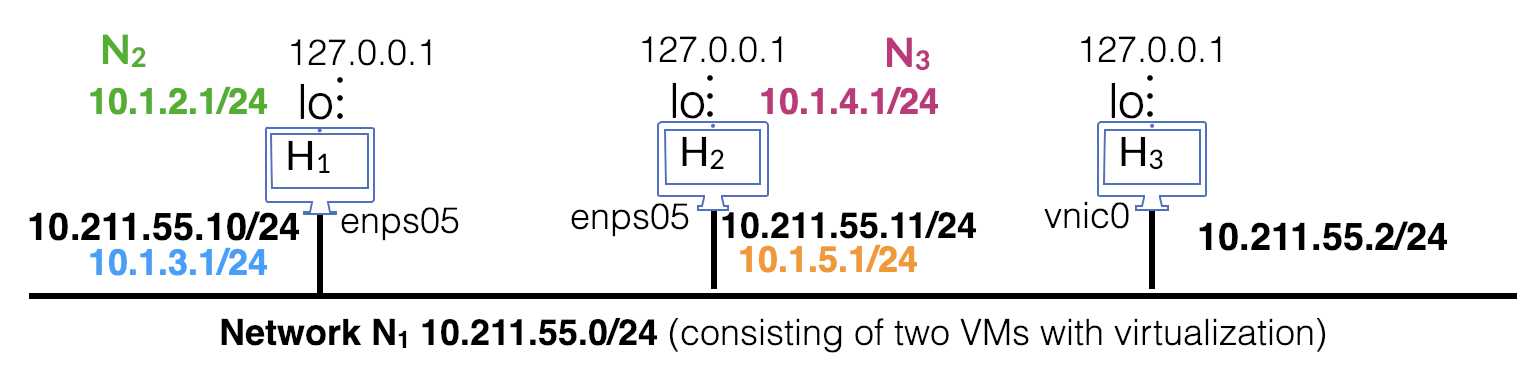
\includegraphics[scale=1.4]{src/Figures/chap2/chap2-fig02.jpg}
\caption{Multi network connectivity using VMs}\label{chap2-fig02}
\end{figure}

\begin{multicols}{2}
From implementation perspective of this network, a typical reader of this article would have access to a single laptop, and thus we will make use of virtual machines to setup such a network. This requires installing some virtualization software, such as VirtualBox\cite{art2-key07}, VMWare\cite{art2-key09}, Parallels\cite{art2-key08} (only for Mac) etc., on the host system (i.e. laptop running Windows, or Macbook etc.). The above depicted network is created using 2 Virtual Machines running Ubuntu\footnote{Any other version of Ubuntu would work equally well.} 16.4LTS (${\rm H}_{1}$) and 18.4LTS (${\rm H}_{2}$) along with the host OS (${\rm H}_{3}$). Author of this article is using Macbook (host ${\rm H}_{3}$) as the host OS and has created the Ubuntu VMs using Parallels\cite{art2-key08} virtualization software. The network 10.211.55.0/24 is created by virtualization software and all VMs attach to this network. Two Ubuntu VMs (${\rm H}_{1}$ and ${\rm H}_{2}$) get their respective network addresses as 10.211.55.10/24 and 10.211.55.11/24 and host system is assigned the IP address 10.211.55.2/24. As all 3 systems belong to same network, these can communicate with each other directly without requiring any connecting router.
\end{multicols}

\vspace{-1.9cm}

\begin{table}[H]
\caption{Assigning Multiple IP Addresses to host ${\rm H}_{1}$}\label{chap2-table-4}
\begin{center}
\begin{tabular}{|l@{\;}l|}
\hline
\# & Assigning addresses to host ${\rm H}_{1}$\\
\# & Addresses on power up of ${\rm H}_{1}$\\
01:& ${\rm H}_{1}$> ip -4 addr show\\
1: & lo: <LOOPBACK,UP,LOWER\_UP> mtu 65536 $\ldots$\\
   & \quad inet 127.0.0.1/8 scope host lo $\ldots$\\
2: & enp0s5: <BROADCAST,MULTICAST,UP,LOWER\_UP> mtu 1500 $\ldots$\\
   & \quad inet 10.211.55.10/24 brd 10.211.55.255 scope global dynamic enp0s5 $\ldots$\\
   \hline
\# & Assigning new network addresses to enp0s5 and lo interface of ${\rm H}_{1}$\\
02:& ${\rm H}_{1}$> sudo ip addr add 10.1.2.1/24 dev lo\\
03:& ${\rm H}_{1}$> sudo ip addr add 10.1.3.1/24 dev enp0s5\\
\hline
\# & Verification of new addresses on ${\rm H}_{1}$\\
04:& ${\rm H}_{1}$> ip -4 addr show\\
1: & lo: <LOOPBACK,UP,LOWER\_UP> mtu 65536 $\ldots$\\
   &\quad inet 127.0.0.1/8 scope host lo $\ldots$\\
   & \quad inet 10.1.2.1/24 scope global lo $\ldots$\\
2: & enp0s5: <BROADCAST,MULTICAST,UP,LOWER\_UP> mtu 1500 $\ldots$\\
   & \quad inet 10.211.55.10/24 brd 10.211.55.255 scope global dynamic enp0s5 $\ldots$\\
   &\quad inet 10.1.3.1/24 scope global enp0s5 $\ldots$\\
   \hline   
\end{tabular}
\end{center}
\end{table}

\vspace{-1.9cm}

\begin{multicols}{2}
Understanding of routing and building a routing table requires us to work with more than one network. Though at the time of VM invocation, they belong to only one network, we will create 4 more networks, and assign two networks to each of Ubuntu VM using its ethernet interface en0s5 as well as loopback lo interface. We will make use of the phenomenon of assigning a number of network addresses (even belonging to different networks) to a network interface.  Table~\ref{chap2-table-4} and Table~\ref{chap2-table-5} respectively provide Linux commands to assign multiple IP addresses to interfaces of hosts ${\rm H}_{1}$ and ${\rm H}_{2}$. Line 01 (Table~\ref{chap2-table-4}) shows the existing IP addresses belong to loopback and ethernet interfaces of host ${\rm H}_{1}$.  Lines 02 and 03 assign the new network addresses respectively to loopback and ethernet interfaces. These new addresses are in addition to existing addresses and same is shown in output of command at line 04. Similarly, lines 01-04 (Table~\ref{chap2-table-5}) shows the assignment of new network addresses to host ${\rm H}_{2}$. The ethernet interface name would vary depending upon VM Ubuntu installation, and thus reader should appropriately replace it in the network setup being created for experiential learning as described in.

With the creation of 4 new networks, host ${\rm H}_{1}$ does not know the route to reach the network 10.1.4.0/24 and 10.1.5.0/24. Similarly, host ${\rm H}_{2}$ does not know how to reach the networks 10.1.2.0/24 and 10.1.3.0/24. Reachability to these networks requires creation of routing entries in the routing tables of ${\rm H}_{1}$ and ${\rm H}_{2}$ respectively. Host ${\rm H}_{1}$ (IP address 10.211.55.10) can reach both 10.211.55.11(${\rm H}_{2}$) and 10.211.55.2(${\rm H}_{3}$) as all three addresses belongs to same network with network number 10.211.55.0/24. Similarly, host ${\rm H}_{2}$ (10.211.55.11) can reach both 10.211.55.10(${\rm H}_{1}$) and 10.211.55.2(${\rm H}_{3}$). The networks 10.1.4.0/24 and 10.1.5.0/24 are reachable via 10.211.55.11(${\rm H}_{2}$) and thus ${\rm H}_{2}$ can act as gateway for these two networks. Similarly, networks 10.1.2.0/24 and 10.1.3.0/24 are reachable via 10.211.55.10 (${\rm H}_{1}$), and thus ${\rm H}_{1}$ can act as gateway for these two networks. 
\end{multicols}

\begin{table}[H]
\caption{Assigning Multiple IP Addresses to Host ${\rm H}_{2}$}\label{chap2-table-5}
\begin{center}
\begin{tabular}{|l@{\;}l|}
\hline
\# & Assigning addresses to host ${\rm H}_{1}$\\
\# & Addresses on power up of ${\rm H}_{1}$\\
01:& ${\rm H}_{2}$ > ip -4 addr\\
1: & lo: <LOOPBACK,UP,LOWER\_UP> mtu 65536 $\ldots$\\
    &\quad inet 127.0.0.1/8 scope host lo $\ldots$\\
2: & enp0s5: <BROADCAST,MULTICAST,UP,LOWER\_UP> mtu 1500 $\ldots$\\
   & \quad inet 10.211.55.11/24 brd 10.211.55.255 scope global $\ldots$ enp0s5 $\ldots$\\
    \hline
\# & Assigning new addresses to enp0s5 and lo interface of ${\rm H}_{2}$\\
02: & ${\rm H}_{2}$ > sudo ip addr add 10.1.4.1/24 dev lo\\
03: & ${\rm H}_{2}$ > sudo ip addr add 10.1.5.1/24 dev enp0s5\\
\hline
\# & Verification of new addresses on ${\rm H}_{2}$\\
04:& ${\rm H}_{2}$ > ip -4 addr\\
1:& lo: <LOOPBACK,UP,LOWER\_UP> mtu 65536 $\ldots$\\
   & \quad inet 127.0.0.1/8 scope host lo $\dots$\\
   &  \quad inet 10.1.4.1/24 scope global lo $\ldots$\\
  \hline 
2:& enp0s5: <BROADCAST,MULTICAST,UP,LOWER\_UP> mtu 1500 $\ldots$\\
   & \quad inet 10.211.55.11/24 brd 10.211.55.255 scope global $\ldots$ enp0s5 $\ldots$\\
   & \quad inet 10.1.5.1/24 scope global enp0s5 $\ldots$\\
   \hline
\end{tabular}
\end{center}
\end{table}

\vspace{-1.1cm}

\begin{multicols}{2}
Using this reachability knowledge of these new networks, routing table entries for these networks on ${\rm H}_{1}$ and ${\rm H}_{2}$ are created using each other as the gateway. The commands to create the routing entries are shown in Table~\ref{chap2-table-6}. The command “ip route add” (lines 02-03) has basically four parameters corresponding to four fields of the routing table (Table~\ref{chap2-table-1}). As ${\rm H}_{1}$ and ${\rm H}_{2}$ are hosts (end systems) and are connected to multiple networks, these systems are known as multi-homed hosts, as a host either consumes (receives) or generates (sends) a packet. To enable routing functionality in a host so that it can forward packets across the connected networks, it needs to be configured as a router i.e. forward packets across interfaces/networks. The commands in Table~\ref{chap2-table-6} at line 01 and 05 enable routing functionality in these two hosts. Line 02 (Table~\ref{chap2-table-6}) adds the routing entry for network 10.1.4.0/24, next hop gateway as 10.211.55.11 (${\rm H}_{2}$) and packet has to be sent out on interface enp0s5. Similarly, command at line 03 adds the routing entry in ${\rm H}_{1}$ for $2^{\rm nd}$ network 10.1.5.0/24. Similarly, lines 06-07 demonstrate creation of routing entries in host ${\rm H}_{2}$.
\end{multicols}

\vspace{-1cm}

\begin{table}[H]
\caption{Creating Routing table}\label{chap2-table-6}
\begin{center}
\begin{tabular}{|l@{\;}l|}
\hline
\# & Creating routing table at ${\rm H}_{1}$\\
01:& ${\rm H}_{1}$> sysctl -w net.ipv4.ip\_forward=1\\
02:& ${\rm H}_{1}$> sudo ip route add 10.1.4.0/24 via 10.211.55.11 dev enp0s5\\
03:& ${\rm H}_{1}$> sudo ip route add 10.1.5.0/24 via 10.211.55.11 dev enp0s5\\
04:& ${\rm H}_{1}$> ip -4 route show\\
   &\quad default via 10.211.55.1 dev enp0s5  proto static metric 100 \\
   &\quad 10.1.3.0/24 dev enp0s5  proto kernel  scope link src 10.1.1.1 \\
   &\quad 10.1.4.0/24 via 10.211.55.11 dev enp0s5 \\
   &\quad 10.1.5.0/24 via 10.211.55.11 dev enp0s5 \\
   &\quad 10.211.55.0/24 dev enp0s5 proto kernel scope link src 10.211.55.10\\
\hline
\# & Creating routing table at ${\rm H}_{2}$\\
05:& ${\rm H}_{2}$> sysctl -w net.ipv4.ip\_forward=1\\
06:& ${\rm H}_{2}$> sudo ip route add 10.1.2.0/24 via 10.211.55.10 dev enp0s5\\
07:& ${\rm H}_{2}$> sudo ip route add 10.1.3.0/24 via 10.211.55.10 dev enp0s5\\
08:& ${\rm H}_{2}$> ip -4 route show\\
   &\quad default via 10.211.55.1 dev enp0s5 proto dhcp metric 100\\ 
   &\quad 10.1.2.0/24 via 10.211.55.10 dev enp0s5\\ 
   &\quad 10.1.3.0/24 via 10.211.55.10 dev enp0s5\\
   &\quad 10.1.5.0/24 dev enp0s5 proto kernel scope link src 10.2.1.1 \\
   &\quad 10.211.55.0/24 dev enp0s5 proto kernel scope link src 10.211.55.11\\
\hline
\end{tabular}
\end{center}
\end{table}

\begin{multicols}{2}
The routing table entries are shown as output of line 04 (host ${\rm H}_{1}$) and 08 (host ${\rm H}_{2}$). Routing entries for ${\rm H}_{1}$ shows that network 10.1.3.0/24 is directly connected using enp0s5 (network interface) and there is no (via) gateway. For networks 10.1.4.0/24 and 10.1.5.0/24, the next hop gateway is 10.211.55.11 (i.e. ${\rm H}_{2}$) reachable via network interface enp0s5. Similarly, line 08 shows the routing entries for host ${\rm H}_{2}$. Now if from ${\rm H}_{1}$, when “ping -c2 10.1.4.1” or “ping -c2 10.1.5.1” is invoked, two ICMP requests will be sent to these addresses via host ${\rm H}_{2}$ and corresponding responses will be received. A successful ping response implies that routing table entries are correct. Ping to any other unassigned network IP address e.g. 10.1.5.2 will result in timeout and no response will be received. It is interesting to know that when an IP address is assigned to a loopback interface in Linux, it automatically assumes that all IP addresses belong to it as well. Thus, when IP address 10.1.4.2 or 10.1.4.200 is pinged from ${\rm H}_{1}$, it will still be successful even though these IP addresses are not directly assigned to loopback interface of ${\rm H}_{2}$ and neither shown (line 04 Table~\ref{chap2-table-5}).

The set of steps for experiential exercise to construct the routing table and its usage in delivering packet to next hop router is given in Exercise~\ref{chap2-exe2}.

\section{Route Aggregation}\label{chap2-sec5}

Internet consists of large number of networks and if a router needs to keep an entry for each network, then number of entries in routing table are likely to exceed millions and thus puts a constraint on memory and compute resources of a router. Routers would like to minimize the number of routing entries and thereby improve upon the packet forwarding performance. The technique to minimize the number of routing entries is achieved by using route aggregation mechanism, in which multiple routing entries are aggregated into a single routing entry. To understand route aggregation mechanism, consider our simple network setup as shown in Figure~\ref{chap2-fig02}. Host ${\rm H}_{2}$ acts as the gateway for 2 networks 10.1.4.0/24 and 10.1.5.0/24 and correspondingly there are 2 routing entries in the routing table of ${\rm H}_{1}$. For the routing purpose from the perspective of ${\rm H}_{1}$, both the networks 10.1.4.0/24 and 10.1.5.0/24 are reachable via gateway ${\rm H}_{2}$. Thus, if these two networks can be aggregated into a single network, ${\rm H}_{1}$ will have only one routing entry for these two networks. These two networks are contiguous, each having 256 IP addresses, and thus can be aggregated as 10.1.4.0/23 representing a total of 512 IP addresses. Thus, a single routing entry can be created using the command “ip route add 10.4.1.0/23 via 10.211.55.11 dev enp0s5”. This technique of using a single subnet prefix (mask) to aggregate and advertise multiple network is also called route summarization or address aggregation.


Address aggregation requires that networks being aggregated should be contiguous and have same number of IP addresses in them. However, though this is a necessary requirement but not sufficient. For example, two networks 10.1.1.0/24 and 10.1.2.0/24 can’t be combined into a single network with a prefix of /23, though both the networks have 256 IP addresses and are contiguous. The summarized network number and the two (or more) networks being combined must have the same higher order bits in the network portion, and should follow the proper hierarchical fashion of address allocation. In this example, first network 10.1.1.0/24 has high order 23 bits as “00001010 00000001 0000000” and the second network 10.1.2.0/24 has high order 23 bits as “00001010 00000001 0000001”. These high order 23 bits differ in last bit i.e. $23^{\rm rd}$ bit which is value 0 for first network and value 1 for the second network. However, since these two networks have high order 22 bits as same i.e.”00001010 00000001 000000”, so one would like to aggregate these as 10.1.0.0/22. This cannot be done since the subnet prefix of /22 will have 10 bits in its host part and thus total number of possible IP addresses in the aggregated network would become 1024.  This would imply that this aggregation will include the network 10.1.0.0/24 as well as the network 10.1.3.0/24, which are not part of original aggregation.

So, requirements for route summarization of N networks are listed as below. 
\begin{itemize}
\item[i.] The number N should be equal to some power k of 2 i.e. N=$2^{\rm k}$ where 0<k<31.
\item[ii.] All the networks should have same number of IP addresses i.e. they should have same subnet prefix (mask) e.g. /m.
\item[iii.] The networks should be contiguous i.e. when the range of IP addresses of one network ends, the next IP address starts the range of next network (being aggregated).
\item[iv.] The high order m-k bits in aggregated network should be same in all individual networks which are being summarized. The subnet prefix of aggregate network would become /m-k i.e. k number of bits will be taken from network part and added to host part. Thus, total number of IP addresses in aggregated network would be equal to $2^{\rm m+k}$.
\end{itemize}

Let us illustrate the summarization process using an example. Consider the following 8 ($=2^{3}$) networks with their representation in bits with network part (highlighted in yellow) and host part (in orange) shown as separated by “|” (and last 3 bits of network parts are underlined and in italics).
\begin{itemize}
\item[i.] 172.16.32.0/23 i.e. 10101100 00010000 0010$\underline{\textit{000}}$ | 0 00000000/23
\item[ii.] 172.16.34.0/23 i.e. 10101100 00010000 0010$\underline{\textit{001}}$ | 0 00000000/23
\item[iii.] 172.16.36.0/23 i.e. 10101100 00010000 0010$\underline{\textit{010}}$ | 0 00000000/23
\item[iv.] 172.16.38.0/23 i.e. 10101100 00010000 0010$\underline{\textit{011}}$ | 0 00000000/23
\item[v.] 172.16.40.0/23 i.e. 10101100 00010000 0010$\underline{\textit{100}}$ | 0 00000000/23
\item[vi.] 172.16.42.0/23 i.e. 10101100 00010000 0010$\underline{\textit{101}}$ | 0 00000000/23
\item[vii.] 172.16.44.0/23 i.e. 10101100 00010000 0010$\underline{\textit{110}}$ | 0 00000000/23
\item[viii.] 172.16.46.0/23 i.e. 10101100 00010000 0010$\underline{\textit{111}}$ | 0 00000000/23
\end{itemize}

The total number of networks are $2^{3}=8$, have same subnet mask of /23, and are contiguous. High order 20 (=23-3) bits are same in all these 8 networks and thus, subnet prefix of aggregated network would be equal to /20 (=23-3), as 3 bits are moved from network part to host part. The new aggregated network number would become 172.16.32.0/20.

When any of the above-mentioned requirement is not satisfied, then networks can’t be aggregated. For example, consider the middle 4 ($=2^{2}$) networks, that is, 172.16.36.0/23, 172.16.38.0/23, 172.16.40.0/23, and 172.16.42.0/23. Thus, the subnet prefix of aggregated network should be /21(=23-2). The $21^{\rm st}$ high order

bit value is 0 in first two networks and has value 1 in the last two networks. Since the last requirement is not met, these 4 networks can’t be aggregated. However, if we consider the first 4 networks, that is, 172.16.32.0/23, 172.16.34.0/23, 172.16.36.0/23 and 172.16.38.0/23, these satisfy all the requirements and thus can be aggregated into the network 172.16.32.0/21. Similarly, if we consider the last 4 networks, that is, 172.16.40.0/23, 172.16.42.0/23, 172.16.44.0/23, and 172.16.46.0/23, these meet all the requirements and can be aggregated as 172.16.40.0/21.

The set of steps for experiential exercise to learn route aggregation and use the route summarization to forward packets in real networks is given in Exercise~\ref{chap2-exe3}.

\section{Longest Prefix Match in Routing Table}\label{chap2-sec6}

Route summarization is typically done when all the networks being aggregated are reachable from same router. This is typically done at ISP (Internet Service Provider) routers. However, at times, some customer of an ISP, which initially belonged to an aggregated network, moves out to another ISP and thus no more reachable by aggregated routing, as it is connected by a different ISP router. Then as per aggregation requirements listed earlier, route summarization fails and number of routing entries increases from 1 summarized entry to many entries corresponding to remaining networks. It is imperative for efficiency reasons to minimize the number of entries in the routing table of a router and thus a router would still prefer to use route summarization though excluding the network which has just moved to a different router. This requirement of still using route summarization to minimize number of routing entries even though some network has moved out of aggregation is served by a routing technique known as Longest Prefix Match.

\begin{figure}[H]
\centering
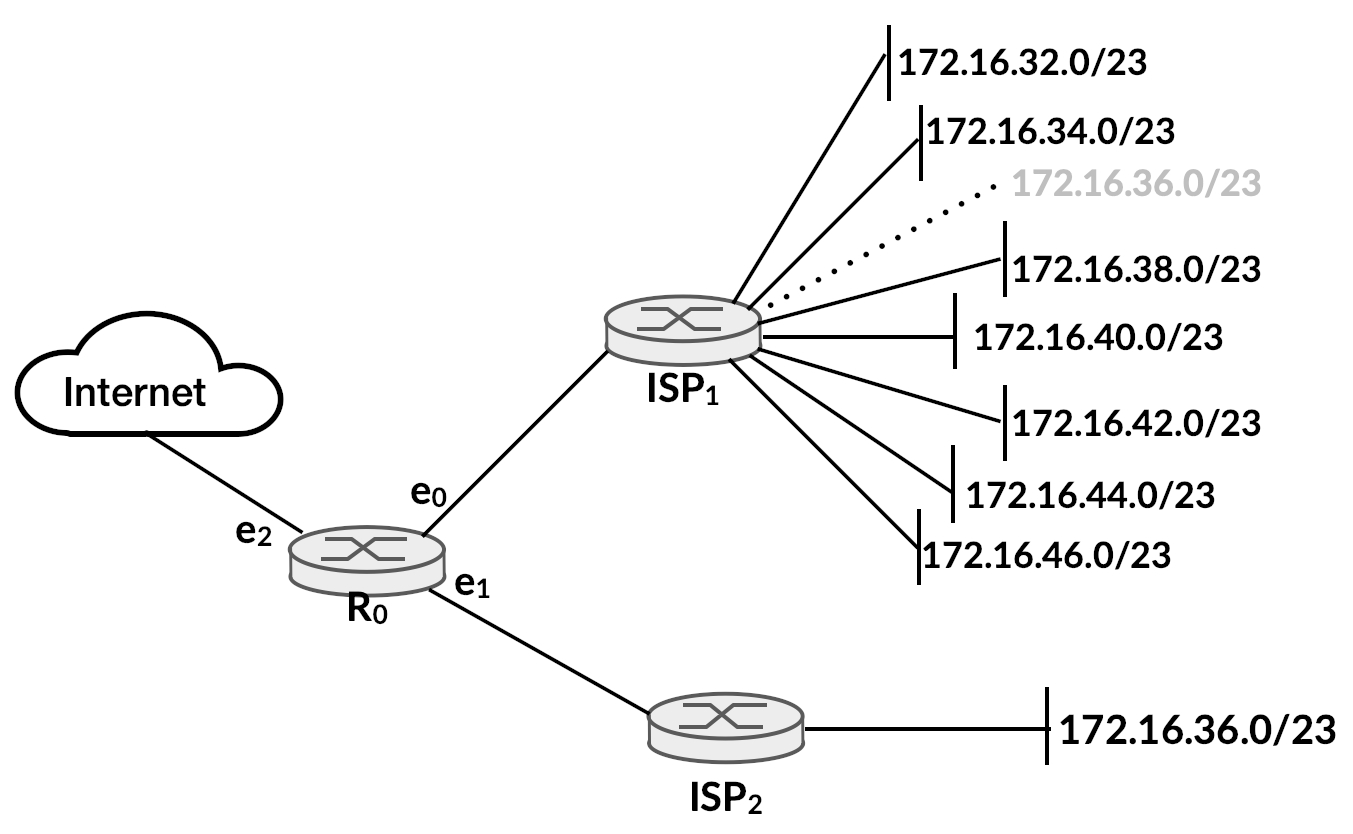
\includegraphics[scale=.8]{src/Figures/chap2/chap2-fig03.jpg}
\caption{Network routing with Longest Prefix Match}\label{chap2-fig03}
\end{figure}

Consider the network as shown in Figure~\ref{chap2-fig03}. One customer network 172.16.36.0/23 has moved from ${\rm ISP}_{1}$ to ${\rm ISP}_{2}$. Before this network movement to ${\rm ISP}_{2}$, all the 8 networks were reachable via router ${\rm ISP}_{1}$.  Thus, router ${\rm R}_{0}$, had a single aggregated routing entry for these 8 networks as destination network/mask: 172.16.32.0/20, next hop: ISP1, and network interface ${\rm e}_{0}$.  After this network moves from ${\rm ISP}_{1}$ to ${\rm ISP}_{2}$, route summarization conditions are violated and thus these can’t be summarized in a single route. So, router ${\rm R}_{0}$ needs to either create individual entries for each of the 7 networks in the routing table, or alternatively partially summarize these creating 4 entries as shown in Table~\ref{chap2-table-7}. Using longest prefix match mechanism, the number of routing entries for these networks can be reduced to 2, one corresponding to aggregated network and one corresponding to the network that has moved out of aggregation as shown in Table~\ref{chap2-table-8}.
\end{multicols}

\begin{table}[H]
\caption{Partial route summarization}\label{chap2-table-7}
\begin{center}
\begin{tabular}{|l|l|l|l|l|}
\hline
\textbf{S.N.} & \textbf{Destination Network} & \textbf{Netmask} & \textbf{Interface} & \textbf{Next Hop}\\
\hline
1 & 172.16.32.0 & /22 & ${\rm e}_{0}$ & ISP1\\
\hline
2 & 172.16.36.0 & /23 & ${\rm e}_{1}$ & ISP2\\
\hline
3 & 172.16.38.0 & /23 & ${\rm e}_{0}$ & ISP1\\
\hline
4 &  172.16.40.0 &  /21 & ${\rm e}_{0}$ & ISP1\\
\hline
$\ldots$ & $\ldots$ & & &\\
\hline
 & 0.0.0.0 & /0 & ${\rm e}_{2}$ & IP address of ${\rm R}_{2}$\\
\hline
\end{tabular}
\end{center}
\end{table}

\vskip -1.2cm

\begin{table}[H]
\caption{Routing Entries Using Longest Prefix Match}\label{chap2-table-8}
\begin{center}
\begin{tabular}{|l|l|l|l|l|}
\hline
\textbf{S.N.} & \textbf{Destination Network} & \textbf{Netmask} & \textbf{Interface} & \textbf{Next Hop}\\
\hline
1 & 172.16.36.0 & /23 & ${\rm e}_{1}$ & ${\rm ISP}_{2}$\\
\hline
2 & 172.16.32.0 & /20 & ${\rm e}_{0}$ & ${\rm ISP}_{1}$\\
\hline
3 & 0.0.0.0 & /0 & ${\rm e}_{2}$ & IP address of ${\rm R}_{2}$\\
\hline
\end{tabular}
\end{center}
\end{table}

\vspace{-1cm}

\begin{multicols}{2}
Consider that Router ${\rm R}_{0}$ gets a packet with destination address of 172.16.36.1. When router ${\rm R}_{0}$ applies routing algorithm as described in to the entries of Table~\ref{chap2-table-8}, row 1 computes the destination network as 172.16.36.0/23 and row 2 computes the destination network as 172.16.32.0/20. Thus, routing algorithm matches both entries corresponding to row 1 and 2, each identifying different next hop router with different network interface. However, a packet can only be forwarded to one of these two next hops and not both. Approach of longest prefix match resolves the issue of multiple matching, and states that choose the routing entry that has the longest prefix (subnet mask) in the $2^{\rm nd}$ column of routing table. Thus, in this case, router ${\rm R}_{0}$ will choose the entry corresponding to prefix /23 rather than /20 since former has longer prefix (23 bits) compared to the latter which has shorter prefix (20 bits). Thus, router ${\rm R}_{0}$ correctly forwards this packet on interface ${\rm e}_{1}$ to next hop router ${\rm ISP}_{2}$. Sequential searching in the routing table to find the entry with longest prefix is optimized by organizing these entries in the routing table starting from longest prefix to shorter prefix. Thus, using routing algorithm, entry with longest prefix will be matched first and packet will be forwarded without even matching with other entries with shorter prefix. However, high end router instead of searching sequentially, use Content Addressable Memories (CAM) technique to search the entries for the given IP Address which perform search in O(1) time rather than O(n) taken by sequential search, and use longest prefix match to select the next hop.

\vspace{-.3cm}

The set of steps for experiential exercise to create the network setup with longest prefix match routing and corresponding forwarding of the packets is described in Exercise~\ref{chap2-exe4}.

\vspace{-.3cm}

\section{Dynamic Routing}\label{chap2-sec7}

\vspace{-.3cm}

So far, we have used static (manual) approach to create routing entries in routing table. This approach works fine when underlying network is of small size, and network topology is fairly static and rarely undergoes any changes. In such networks, any topology change occurs over a longer period of time e.g. few months or even years. For example, a college network generally does not undergo any changes unless a new laboratory or department is created or course contents are modified which occur mostly on yearly basis. Creation of manual entries does not work for a large network, as entries have to be manually created for all the routers in the network.  When configuring large number of routers with manual entries, chance of making a configuration error is quite high and it take humongous efforts to identify and rectify such configuration errors. Further, larger network would undergo changes more frequently, such as, a link going down or coming back up or a router crashing, etc.  Any such change in network topology would require updates in routing tables of all routers in the network which is a tedious task, likely to cause more manual errors and thus neither manageable nor scalable.


In larger size networks, routers use routing protocols to create the routing tables automatically. Routers exchange information about connected and reachable networks with other routers, and build their routing table. Any change in network topology e.g. a link going down or coming back up, a new router being added into the network or some working router going down is detected by neighbouring routers of the affected link/router. This topology change results in immediate exchange of routing information by neighbouring routers to other routers and eventually percolated to all routers in the network. Thus, in a short time (known as convergence time), all routers of network get the routing update about the changes in network topology and update their routing table. These routing protocols are classified into two categories  \cite{art2-key10}, a) Link State Routing, and b) Distance Vector Routing. Open Shortest Path First (OSPF)\cite{art2-key04} is a link state routing protocol which is widely implemented by many network administrators. Routing Information Protocol (RIP) \cite{art2-key05}\cite{art2-key06} implements distance vector routing approach and was the routing protocol which was first implemented and distributed as part of BSD Unix (Berkeley System Division Unix) distribution. It is practically infeasible to build a real live network to explore dynamic routing protocols using experiential learning as it would involve setting up of fairly sufficient number of systems and routers, to which reader of this article may not have access. Interested readers are requested to explore these by going through references and text books on networks and understand working of dynamic routing protocols.

\section{Summary}\label{chap2-sec8}

We have discussed need of IP routing to deliver packets from one system to another, when these are connected either directly on the same network or via a number of intermediate routers. Each router as well as a host in the network maintains a routing table, and uses routing algorithm to forward packets.  A typical routing table needs minimum of 4 entries, namely a) destination network, b) netmask (or prefix), c) network interface, and d) IP address of next hop router. Routing table needs to have one entry for each of the network number present in the network setup. Generally, a routing table also has a default entry as 0.0.0.0/0 so that that it matches all destinations. We have also explored the need of ARP protocol to map an IP address to MAC address as latter is needed by link layer adaptor to receive and process the frame and pass the extracted network packet to higher layer network stack in the system for further processing. When a packet is forwarded by one intermediate router to next, it does not change source and destination IP address as provided originally by the sender host. The delivery to next hop is achieved by adding the destination MAC address of next hop router by the previous router/host in the path from source to destination. As internet consists of a large number of networks, technique of route summarization (also called as route aggregation) is used to summarize multiple routing entries in a single route to minimize the number of routing entries to improve the routing performance. We have also discussed use of longest prefix match to correctly route the packets when some networks that were part of route aggregation, move to a different router.

\section{Experiential Exercises}\label{chap2-sec9}

To understand and learn IP routing experientially, an experimental setup similar to the one shown in Figure~\ref{chap2-fig02} is used for hands-on exercises. One can either use 3 independent systems, or using a single system, create two Ubuntu VMs (Virtual Machine) using virtualization software \cite{art2-key07}\cite{art2-key08}\cite{art2-key09} to create such a network. The host OS (that runs virtualization application) can be Windows, Macbook or Linux. In the exercises described below, the network number used by VMs is shown as 10.211.55.0/24 and this may vary depending upon the setup creation. So, the IP address belonging to this network should be appropriately modified as per the VM setup (for example, it may have 192.168.x.0/24 network number for some x, 0<=x<=255) that a learner would create. Similarly, network interface names may have to appropriately replaced as per the network interface names in the setup created by the learner. The new networks used in experiential learning of IP routing can either be used as shown in Figure~\ref{chap2-fig02}, that is, 10.1.y.0 (2<=y<=5) or modify it as desired. In the exercises described below, the IP addresses and network interface names of host OS (MacOS), VM1(Ubuntu 16)/enp0s5 and VM2(Ubuntu 18)/enp0s5 are corresponding used as (vnic0)10.211.55.2/24, (enp0s5)10.211.55.10/24 and (enp0s5)10.211.55.11/24. The IP address of gateway router that will connect to internet using the host OS is 10.211.55.1/24.

To understand the working of IP routing and ARP protocol, run wireshark on both ${\rm H}_{1}$ and ${\rm H}_{2}$ and capture packets for IP addresses of source and destination addresses used for communication.


\section*{Exercise \thnum{1}\label{chap2-exe1}}

\textbf{Topic: Routing and delivery of packets when two systems are connected directly on a network}

\vspace{-.5cm}

\begin{itemize}
\item[a] Power on ${\rm H}_{1}$ (${\rm VM}_{1}$-Ubuntu) and login into ${\rm H}_{1}$.
\item[b] Find out the IP addresses of both loopback and ethernet interfaces. The loopback (lo) interface would always have IP address as 127.0.0.1 and ethernet (enp0s5) would have IP address like 10.211.55.10/24 (this IP address may vary depending upon the VM network being used). Use the command below to find the IP Addresses (shows in highlighted yellow)

	\textbf{H1> ip -4 addr show}

	1: lo: <LOOPBACK,UP,LOWER\_UP> mtu 65536 qdisc noqueue state UNKNOWN group default qlen 1

	inet 127.0.0.1/8 scope host lo

	valid\_lft forever preferred\_lft forever

	2: enp0s5: 
	
	<BROADCAST,MULTICAST,UP,LOWER\_UP>\break mtu 1500 qdisc pfifo\_fast state UP group default qlen 1000

	inet 10.211.55.10/24 brd 10.211.55.255 scope global dynamic enp0s5

	valid\_lft 1718sec preferred\_lft 1718sec


\item[c.] Analyze the routing table entries. It should have basically two entries. First one for default destination (0.0.0.0/0) with the next hop as gateway (via) address 10.211.55.1 and second one belonging to local (VM) network 10.211.55.0/24 without any next hop (via). Use the command below to find the routing information (destination network is shown in highlighted yellow)

	${\rm H}_{1}$> \textbf{ip -4 route show}

	default via 10.211.55.1 dev enp0s5 proto static  metric 100

	10.211.55.0/24 dev enp0s5 proto kernel scope link src 10.211.55.10

	metric 100

	169.254.0.0/16 dev enp0s5 scope link  metric 1000

\item[d.] Analyze the ARP table entries. It should basically have one entry corresponding to default gateway 10.211.55.1. Use the command below to find ARP table entries. The MAC address corresponding to default gateway would vary as per network setup. Depending upon the network activity it may show more entries as well.

	H1> \textbf{arp -an}

	? (10.211.55.1) at 00:1c:42:00:00:18 [ether] on enp0s5

\item[e.]  Power on ${\rm H}_{2}$ (${\rm VM}_{2}$-Ubuntu) and repeat the steps described above to find the IP address (10.211.55.11), routing table information (two entries one for default network (0.0.0.0/0) with default gateway as 10.211.55.1, and one for locally connected network 10.211.55.0/24) and ARP entries (one entry for default gateway 10.211.55.1). Use the command below to find these information

	${\rm H}_{2}$ > \textbf{ip -4 addr show}

	1: lo : <LOOPBACK,UP,LOWER\_UP> mtu 65536 qdisc noqueue state UNKNOWN group default qlen 1000

	inet 127.0.0.1/8 scope host lo

	valid\_lft forever preferred\_lft forever

	2: enp0s5: <BROADCAST,MULTICAST,UP,LOWER\_UP> mtu 1500 qdisc fq\_codel state UP group default qlen 1000

	inet 10.211.55.11/24 brd 10.211.55.255 scope global dynamic noprefixroute enp0s5

	valid\_lft 1506sec preferred\_lft 1506sec

	${\rm H}_{2}$ > \textbf{ip -4 route show}

	default via 10.211.55.1 dev enp0s5 proto dhcp metric 100

	10.211.55.0/24 dev enp0s5 proto kernel scope link src 10.211.55.11

	metric 100

	169.254.0.0/16 dev enp0s5 scope link metric 1000

	${\rm H}_{2}$ > \textbf{arp -an}

	? (10.211.55.1) at 00:1c:42:00:00:18 [ether] on enp0s5

\item[f.] Launch wireshark on ${\rm H}_{1}$ and capture traffic for ${\rm H}_{2}$, and launch wireshark on ${\rm  H}_{2}$ to capture traffic for ${\rm H}_{1}$.

\item[g.] From ${\rm H}_{1}$ (10.211.55.10), send two ping packets to ${\rm H}_{2}$ (10.211.55.11) using the command below

	${\rm H}_{1}$ > \textbf{ping -c2 10.211.55.11}

\item[h.]  Verify ping command is successful i.e. ${\rm H}_{1}$ receives ping response.
\item[i.] Analyze the ARP table on ${\rm H}_{1}$. It should show ARP entry for ${\rm H}_{2}$.

	${\rm H}_{1}$ > \textbf{arp -an}

\item[j.] Analyze the ARP table on ${\rm H}_{2}$. It should show ARP entry for ${\rm H}_{1}$.

	${\rm H}_{2}$ > arp -an

\item[k.] Using wireshark, verify the ARP broadcast request from ${\rm H}_{1}$ (10.211.55.10) to know who is 10.211.55.11 and ARP unicast reply from ${\rm H}_{2}$ (10.211.55.11) to ${\rm H}_{1}$.
\end{itemize}

\textbf{Learning:} Working of ARP protocol for delivering packets in locally connected network.

\section*{Exercise \thnum{2}}\label{chap2-exe2}

\textbf{Topic: Routing and delivery of packets when two networks are connected by intermediate routers.}

\begin{itemize}
\item[a.] Create a new network 10.1.2.0/24 and assign 10.1.2.1/24 in this network to ethernet interface of ${\rm H}_{1}$

${\rm H}_{1}$ > \textbf{sudo ip addr add 10.1.2.1/24 dev enp0s5}

\item[b.] Create a new network 10.1.4.0/24 and assign 10.1.4.1/24 in this network to ethernet interface of ${\rm H}_{2}$

${\rm H}_{2}$ > \textbf{sudo ip addr add 10.1.4.1/24 dev enp0s5}

\item[c.] Since both ${\rm H}_{1}$ and ${\rm H}_{2}$ now connects two networks and thus can act as routers. Enable routing functionalities in these multi-homed hosts using the following command. (Please note there should not be any SPACE character before and after ‘=’ (equal) sign.

${\rm H}_{1}$ > \textbf{sudo sysctl -w net.ipv4.ip\_forward=1}

${\rm H}_{2}$ > \textbf{sudo sysctl -w net.ipv4.ip\_forward=1}

\item[d.] Make a routing entry for network 10.1.2.0/24 (connected via ${\rm H}_{1}$) in the routing table of ${\rm H}_{2}$.

${\rm H}_{2}$ > \textbf{sudo ip route add 10.1.2.0/24 via 10.211.55.10 dev enp0s5}

\item[e.] Make a routing entry for network 10.1.4.0/24 (connected via ${\rm H}_{2}$) in the routing table of ${\rm H}_{1}$.

${\rm H}_{1}$ > \textbf{sudo ip route add 10.1.4.0/24 via 10.211.55.11 dev enp0s5}

\item[f.] Run wireshark on both H1 and H2 and capture traffic respectively for 10.1.2.1 and 10.1.4.1.

\item[g.] From ${\rm H}_{1}$, sending two ping packets to newly assigned $2^{\rm nd}$ IP address of ${\rm H}_{2}$ (10.1.4.1)

${\rm H}_{1}$ > \textbf{ping -c2 10.1.4.1}


\item[h.] From ${\rm H}_{2}$, sending two ping packets to newly assigned $2^{\rm nd}$ IP address of ${\rm H}_{1}$ (10.1.2.1)

${\rm H}_{2}$ > \textbf{ping -c2 10.1.2.1}

\item[i.] Both ping requests should be successful.

\item[j.] There should not be any new ARP entries in the ARP Table. ${\rm H}_{1}$ would have ARP entry for ${\rm H}_{2}$ (10.211.55.11) as gateway for network 10.1.4.0/24, and ${\rm H}_{2}$ should have ARP entry for ${\rm H}_{1}$ (10.211.55.10) as gateway for network. 10.1.2.0/24.


\item[k.] Analyze the ping packets in wireshark captures and verify the source and destination IP addresses as well as source and destination MAC addresses.

\item[i.] Remove the routing entries created above in $4^{\rm th}$ and $5^{\rm th}$ step.

${\rm H}_{1}$ > \textbf{sudo ip route del 10.1.4.0/24 via 10.211.55.11 dev enp0s5}

${\rm H}_{2}$ > \textbf{sudo ip route del 10.1.2.0/24 via 10.211.55.10 dev enp0s5}

\item[m.] Send the ping packets again from ${\rm H}_{1}$ to 10.1.4.1 and from ${\rm H}_{2}$ to 10.1.2.1. Both pings should fail. This demonstrates the need of proper routing table to send packets.

\end{itemize}

\textbf{Learning:} Use of routing table in forwarding the packets.

\section*{Exercise \thnum{3}\label{chap2-exe3}}

\textbf{Topic: Use of route summarization}

\begin{itemize}
\item[a.] Create a new network 10.1.3.0/24 (that can be route summarized with 10.1.2.0/24) and assign 10.1.3.1/24 in this network to loopback interface lo (or alternately to the ethernet interface enp0s5).

${\rm H}_{1}$ > \textbf{sudo ip addr add 10.1.3.1/24 dev lo}

\item[b.] Create a new network 10.1.5.0/24 (that can be route summarized with 10.1.4.0/24) and assign 10.1.5.1/24 in this network to loopback interface lo (or ethernet interface).

${\rm H}_{2}$ > \textbf{sudo ip addr add 10.1.5.1/24 dev lo}

\item[c.] Create route summarization entry 10.1.2.0/23 corresponding to two networks 10.1.2.0/24 and 10.1.3.0/24 in ${\rm H}_{2}$.

${\rm H}_{2}$ > \textbf{sudo ip route add 10.1.2.0/23 via 10.211.55.10 dev enp0s5}

\item[d.] Create route summarization entry 10.1.4.0/23 corresponding to two networks 10.1.4.0/24 and 10.1.5.0/24 in ${\rm H}_{1}$.

${\rm H}_{1}$ > \textbf{sudo ip route add 10.1.4.0/23 via 10.211.55.11 dev enp0s5}

\item[e.] Send ping packets from ${\rm H}_{1}$ to both new network IP addresses of ${\rm H}_{2}$. 

${\rm H}_{1}$ > \textbf{ping -c2 10.1.4.1}

${\rm H}_{1}$ > \textbf{ping -c2 10.1.5.1}

\item[f.] Send ping packets from ${\rm H}_{2}$ to both new network IP addresses of ${\rm H}_{1}$

${\rm H}_{2}$  > \textbf{ping -c2 10.1.2.1}

${\rm H}_{2}$  > \textbf{ping -c2 10.1.3.1}

\item[g.] All pings should be successful. Analyze the ping packets in wireshark captures w.r.t. their source and destination IP addresses.

\item[h.] Remove the routing entry in ${\rm H}_{2}$ as created in $3^{\rm rd}$ step above.

${\rm H}_{2}$ > \textbf{sudo ip route del 10.1.2.0/23 via 10.211.55.10 dev enp0s5}

\item[i.] Resend the ping packets ($5^{\rm th}$ and $6^{\rm th}$ step). These pings should be unsuccessful. From ${\rm H}_{1}$, packets will reach ${\rm H}_{2}$ (verify in wireshark capture) but ${\rm H}_{2}$ does not have routing entries for reply packets.  Similarly, ${\rm H}_{2}$ will not send Ping request packets to ${\rm H}_{1}$ because of no routing entries. A close analysis in wireshark will show that both these packets follow the default route i.e. these will go to gateway 10.211.55.1 which will be discarded, since these can’t be delivered.
\end{itemize}

\textbf{Learning:} Use of route summarization to reduce the number of routing entries.

\section*{Exercise \thnum{4}\label{chap2-exe4}}

\textbf{Topic: Use of Longest Prefix Match}

\begin{itemize}
\item[a.] Repeat the steps a. to f. from  Exercise~\ref{chap2-exe2} i.e. assign IP address 10.1.2.1/24 to network interface enp0s5 of ${\rm H}_{1}$, and IP address 10.1.4.1 to network interface enp0s5 of ${\rm H}_{2}$, create corresponding routing table and check reachability.

\item[b.] Assign IP address 10.1.2.65/26 to network interface enp0s5 of ${\rm H}_{2}$. Ensure to use the subnet mask /26 which makes a subnet of the network 10.1.2.0/24 belonging to ${\rm H}_{1}$. So essentially, for ${\rm H}_{2}$, aggregated network 10.1.2.0/24 is reachable via ${\rm H}_{1}$, but its small subnet 10.1.2.64/26 is connected via ${\rm H}_{2}$.

\item[c.] Similarly, assign IP address 10.1.4.129/27 to network interface enp0s5 of ${\rm H}_{1}$. Please use the subnet mask /27 which makes a subnet of network 10.1.4.0/24 belonging to ${\rm H}_{2}$. Essentially, for ${\rm H}_{1}$, aggregated network 10.1.4.0/24 is reachable via ${\rm H}_{2}$, but a small subnet 10.1.4.128/27 of it is connected via ${\rm H}_{1}$.

\item[d.] Thus, if from ${\rm H}_{2}$, when IP address 10.1.2.65 is pinged, the longest prefix match will send the packet locally to ${\rm H}_{2}$ and this packet will not go to ${\rm H}_{1}$. However, when IP address 10.1.2.1 is pinged, packet will actually go out on the network interface and reach ${\rm H}_{1}$ and response will be received. Issue the following ping commands and verify these are successful.

${\rm H}_{2}$ > \textbf{ping -c2 10.1.2.65}

${\rm H}_{2}$ > \textbf{ping -c2 10.1.2.1}

\item[e.] Analyze the wireshark capture and verify working of longest prefix match.

\item[f.] Similarly, from ${\rm H}_{1}$, send ping packets to 10.1.4.129 and 10.1.4.1 and verify working of the longest prefix match.

${\rm H}_{1}$ > \textbf{ping -c2 10.1.4.129}

${\rm H}_{1}$ > \textbf{ping -c2 10.1.4.1}

\item[g.] Analyze the wireshark capture and explore working of longest prefix match.
\end{itemize}

\textbf{Learning:} Use of longest prefix match in routing table to route the packets correctly even when multiple match occurs in routing table.

Note: For any clarifications, inputs, suggestions, author can be reached at \url{prustagi@ksit.edu.rin} \raisebox{-.1cm}{
\includegraphics[scale=.9]{src/Figures/circledC.eps}}

\begin{thebibliography}{99}

\bibitem{art2-key01} Ram Rustagi, “Experiential Learning of Networking Technologies: Understanding Network Layer and IP addressing”, journal of Computing and Communications, issue 02 – Vol 04: June 2020,

\url{“https://journal.accsindia.org/understanding-network-layer-ip-addressing/“},

Last accessed Sep 2020.

\bibitem{art2-key02} RFC 791, “Internet Protocol: DARPA Internet Program Protocol Specification”, September 1981,

\url{ https://tools.ietf.org/html/rfc791}.

\bibitem{art2-key03} RFC 862, “An Ethernet Address Resolution Protocol”, Nov 1982, 

\url{https://tools.ietf.org/html/rfc826},

last accessed September 2020.

\bibitem{art2-key04} RFC 1583, “OSPF Version 2”, March 1994,

\url{ https://tools.ietf.org/html/rfc1583},

last accessed September 2020.

\bibitem{art2-key05} RFC 1058, “Routing Information Protocol”, June 1988,

\url{https://tools.ietf.org/html/rfc1058}.

\bibitem{art2-key06} RFC 2453, “RIP Version 2”, November 1998, 

\url{https://tools.ietf.org/html/rfc2453}.

\bibitem{art2-key07} VirtualBox, a powerful virtualization product,

\url{https://www.virtualbox.org},

last accessed September 2020.

\bibitem{art2-key08} Parallels, The most powerful application to run Wndows/Ubuntu on Mac,

\url{https://www.parallels.com},

last accessed September 2020.

\bibitem{art2-key09} VMware Workstation: A desktop virtualization application for personal use,

\url{https://www.vmware.com/in/products/player/faqs.html},

last accessed September 2020.

\bibitem{art2-key10} Kurose, Ross, “Computer Networking: A Top Down Approach”, section 4.5, $6^{\rm th}$ edition, Pearson.

\end{thebibliography}

\end{multicols}


\noindent
\begin{tabular}{V{2.5}cp{14.2cm}V{2.5}}
\clineB{1-2}{2.5}
 &\\
\raisebox{-4cm}{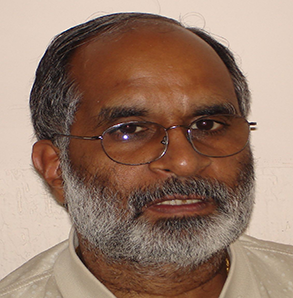
\includegraphics{src/Figures/authors/Rustagi_RPR-PP-Photo.png}} & 

\centerline{\large\bf Prof. Ram P. Rustagi}

\bigskip
Dr.~Ram P. Rustagi is currently working as Professor, CSE dept, KSIT Bangalore, and honed up his academic skills with Ph.D from IIT Delhi, and M.Tech from IISc Bangalore. Prior to KSIT, at Cavisson Systems, he mentored new technology development using Machine Learning techniques in Security and Performance Monitoring. At PES University, he had taught Undergraduates, Post Graduates students, and successfully guided 3 Ph.D scholars. At PESU, he brought innovations in teaching computer network and security courses, and introduced practical experiential learning exercises.\\
&\\ 
\clineB{1-2}{2.5}
\end{tabular}
